%%%%%%%%%%%%%%%%%%%%%%%%%%%%%%%%%%%%%%%%%
% A compendium for the course IBE115 at Molde University College
%
% It contains additions and corrections to the book "Linux tjenestedrift"
%
% Author: Hans Fredrik Nordhaug (hans.f.nordhaug@himolde.no / hansfn@gmail.com)
%
% The structure of the document is based on the "The Legrand Orange Book"
% LaTeX Template, Version 2.2 (30/3/17) downloaded from
% http://www.LaTeXTemplates.com
%
% This document and the template it is based on is licensed under
% CC BY-NC-SA 3.0 (http://creativecommons.org/licenses/by-nc-sa/3.0/)
%%%%%%%%%%%%%%%%%%%%%%%%%%%%%%%%%%%%%%%%%

%----------------------------------------------------------------------------------------
%	PACKAGES AND OTHER DOCUMENT CONFIGURATIONS
%----------------------------------------------------------------------------------------

\documentclass[11pt,fleqn,norsk]{book} % Default font size and left-justified equations

%----------------------------------------------------------------------------------------

%%%%%%%%%%%%%%%%%%%%%%%%%%%%%%%%%%%%%%%%%
% The Legrand Orange Book
% Structural Definitions File
% Version 2.0 (9/2/15)
%
% Original author:
% Mathias Legrand (legrand.mathias@gmail.com) with modifications by:
% Vel (vel@latextemplates.com)
% 
% This file has been downloaded from:
% http://www.LaTeXTemplates.com
%
% License:
% CC BY-NC-SA 3.0 (http://creativecommons.org/licenses/by-nc-sa/3.0/)
%
%%%%%%%%%%%%%%%%%%%%%%%%%%%%%%%%%%%%%%%%%

%----------------------------------------------------------------------------------------
%	VARIOUS REQUIRED PACKAGES AND CONFIGURATIONS
%----------------------------------------------------------------------------------------

\usepackage[top=3cm,bottom=3cm,left=3cm,right=3cm,headsep=10pt,a4paper]{geometry} % Page margins

\usepackage{graphicx} % Required for including pictures
\graphicspath{{Pictures/}} % Specifies the directory where pictures are stored

\usepackage{lipsum} % Inserts dummy text

\usepackage{tikz} % Required for drawing custom shapes

\usepackage[english]{babel} % English language/hyphenation

\usepackage{enumitem} % Customize lists
\setlist{nolistsep} % Reduce spacing between bullet points and numbered lists

\usepackage{booktabs} % Required for nicer horizontal rules in tables

\usepackage{xcolor} % Required for specifying colors by name
\definecolor{ocre}{RGB}{243,102,25} % Define the orange color used for highlighting throughout the book

%----------------------------------------------------------------------------------------
%	FONTS
%----------------------------------------------------------------------------------------

\usepackage{avant} % Use the Avantgarde font for headings
%\usepackage{times} % Use the Times font for headings
\usepackage{mathptmx} % Use the Adobe Times Roman as the default text font together with math symbols from the Sym­bol, Chancery and Com­puter Modern fonts

\usepackage{microtype} % Slightly tweak font spacing for aesthetics
\usepackage[utf8]{inputenc} % Required for including letters with accents
\usepackage[T1]{fontenc} % Use 8-bit encoding that has 256 glyphs

%----------------------------------------------------------------------------------------
%	BIBLIOGRAPHY AND INDEX
%----------------------------------------------------------------------------------------

\usepackage[style=alphabetic,citestyle=alphabetic,sorting=nyt,sortcites=true,autopunct=true,babel=hyphen,hyperref=true,abbreviate=false,backref=true,backend=biber]{biblatex}
\addbibresource{bibliography.bib} % BibTeX bibliography file
\defbibheading{bibempty}{}

\usepackage{calc} % For simpler calculation - used for spacing the index letter headings correctly
\usepackage{makeidx} % Required to make an index
\makeindex % Tells LaTeX to create the files required for indexing

%----------------------------------------------------------------------------------------
%	MAIN TABLE OF CONTENTS
%----------------------------------------------------------------------------------------

\usepackage{titletoc} % Required for manipulating the table of contents

\contentsmargin{0cm} % Removes the default margin

% Part text styling
\titlecontents{part}[0cm]
{\addvspace{20pt}\centering\large\bfseries}
{}
{}
{}

% Chapter text styling
\titlecontents{chapter}[1.25cm] % Indentation
{\addvspace{12pt}\large\sffamily\bfseries} % Spacing and font options for chapters
{\color{ocre!60}\contentslabel[\Large\thecontentslabel]{1.25cm}\color{ocre}} % Chapter number
{\color{ocre}}  
{\color{ocre!60}\normalsize\;\titlerule*[.5pc]{.}\;\thecontentspage} % Page number

% Section text styling
\titlecontents{section}[1.25cm] % Indentation
{\addvspace{3pt}\sffamily\bfseries} % Spacing and font options for sections
{\contentslabel[\thecontentslabel]{1.25cm}} % Section number
{}
{\hfill\color{black}\thecontentspage} % Page number
[]

% Subsection text styling
\titlecontents{subsection}[1.25cm] % Indentation
{\addvspace{1pt}\sffamily\small} % Spacing and font options for subsections
{\contentslabel[\thecontentslabel]{1.25cm}} % Subsection number
{}
{\ \titlerule*[.5pc]{.}\;\thecontentspage} % Page number
[]

% List of figures
\titlecontents{figure}[0em]
{\addvspace{-5pt}\sffamily}
{\thecontentslabel\hspace*{1em}}
{}
{\ \titlerule*[.5pc]{.}\;\thecontentspage}
[]

% List of tables
\titlecontents{table}[0em]
{\addvspace{-5pt}\sffamily}
{\thecontentslabel\hspace*{1em}}
{}
{\ \titlerule*[.5pc]{.}\;\thecontentspage}
[]

%----------------------------------------------------------------------------------------
%	MINI TABLE OF CONTENTS IN PART HEADS
%----------------------------------------------------------------------------------------

% Chapter text styling
\titlecontents{lchapter}[0em] % Indenting
{\addvspace{15pt}\large\sffamily\bfseries} % Spacing and font options for chapters
{\color{ocre}\contentslabel[\Large\thecontentslabel]{1.25cm}\color{ocre}} % Chapter number
{}  
{\color{ocre}\normalsize\sffamily\bfseries\;\titlerule*[.5pc]{.}\;\thecontentspage} % Page number

% Section text styling
\titlecontents{lsection}[0em] % Indenting
{\sffamily\small} % Spacing and font options for sections
{\contentslabel[\thecontentslabel]{1.25cm}} % Section number
{}
{}

% Subsection text styling
\titlecontents{lsubsection}[.5em] % Indentation
{\normalfont\footnotesize\sffamily} % Font settings
{}
{}
{}

%----------------------------------------------------------------------------------------
%	PAGE HEADERS
%----------------------------------------------------------------------------------------

\usepackage{fancyhdr} % Required for header and footer configuration

\pagestyle{fancy}
\renewcommand{\chaptermark}[1]{\markboth{\sffamily\normalsize\bfseries\chaptername\ \thechapter.\ #1}{}} % Chapter text font settings
\renewcommand{\sectionmark}[1]{\markright{\sffamily\normalsize\thesection\hspace{5pt}#1}{}} % Section text font settings
\fancyhf{} \fancyhead[LE,RO]{\sffamily\normalsize\thepage} % Font setting for the page number in the header
\fancyhead[LO]{\rightmark} % Print the nearest section name on the left side of odd pages
\fancyhead[RE]{\leftmark} % Print the current chapter name on the right side of even pages
\renewcommand{\headrulewidth}{0.5pt} % Width of the rule under the header
\addtolength{\headheight}{2.5pt} % Increase the spacing around the header slightly
\renewcommand{\footrulewidth}{0pt} % Removes the rule in the footer
\fancypagestyle{plain}{\fancyhead{}\renewcommand{\headrulewidth}{0pt}} % Style for when a plain pagestyle is specified

% Removes the header from odd empty pages at the end of chapters
\makeatletter
\renewcommand{\cleardoublepage}{
\clearpage\ifodd\c@page\else
\hbox{}
\vspace*{\fill}
\thispagestyle{empty}
\newpage
\fi}

%----------------------------------------------------------------------------------------
%	THEOREM STYLES
%----------------------------------------------------------------------------------------

\usepackage{amsmath,amsfonts,amssymb,amsthm} % For math equations, theorems, symbols, etc

\newcommand{\intoo}[2]{\mathopen{]}#1\,;#2\mathclose{[}}
\newcommand{\ud}{\mathop{\mathrm{{}d}}\mathopen{}}
\newcommand{\intff}[2]{\mathopen{[}#1\,;#2\mathclose{]}}
\newtheorem{notation}{Notation}[chapter]

% Boxed/framed environments
\newtheoremstyle{ocrenumbox}% % Theorem style name
{0pt}% Space above
{0pt}% Space below
{\normalfont}% % Body font
{}% Indent amount
{\small\bf\sffamily\color{ocre}}% % Theorem head font
{\;}% Punctuation after theorem head
{0.25em}% Space after theorem head
{\small\sffamily\color{ocre}\thmname{#1}\nobreakspace\thmnumber{\@ifnotempty{#1}{}\@upn{#2}}% Theorem text (e.g. Theorem 2.1)
\thmnote{\nobreakspace\the\thm@notefont\sffamily\bfseries\color{black}---\nobreakspace#3.}} % Optional theorem note
\renewcommand{\qedsymbol}{$\blacksquare$}% Optional qed square

\newtheoremstyle{blacknumex}% Theorem style name
{5pt}% Space above
{5pt}% Space below
{\normalfont}% Body font
{} % Indent amount
{\small\bf\sffamily}% Theorem head font
{\;}% Punctuation after theorem head
{0.25em}% Space after theorem head
{\small\sffamily{\tiny\ensuremath{\blacksquare}}\nobreakspace\thmname{#1}\nobreakspace\thmnumber{\@ifnotempty{#1}{}\@upn{#2}}% Theorem text (e.g. Theorem 2.1)
\thmnote{\nobreakspace\the\thm@notefont\sffamily\bfseries---\nobreakspace#3.}}% Optional theorem note

\newtheoremstyle{blacknumbox} % Theorem style name
{0pt}% Space above
{0pt}% Space below
{\normalfont}% Body font
{}% Indent amount
{\small\bf\sffamily}% Theorem head font
{\;}% Punctuation after theorem head
{0.25em}% Space after theorem head
{\small\sffamily\thmname{#1}\nobreakspace\thmnumber{\@ifnotempty{#1}{}\@upn{#2}}% Theorem text (e.g. Theorem 2.1)
\thmnote{\nobreakspace\the\thm@notefont\sffamily\bfseries---\nobreakspace#3.}}% Optional theorem note

% Non-boxed/non-framed environments
\newtheoremstyle{ocrenum}% % Theorem style name
{5pt}% Space above
{5pt}% Space below
{\normalfont}% % Body font
{}% Indent amount
{\small\bf\sffamily\color{ocre}}% % Theorem head font
{\;}% Punctuation after theorem head
{0.25em}% Space after theorem head
{\small\sffamily\color{ocre}\thmname{#1}\nobreakspace\thmnumber{\@ifnotempty{#1}{}\@upn{#2}}% Theorem text (e.g. Theorem 2.1)
\thmnote{\nobreakspace\the\thm@notefont\sffamily\bfseries\color{black}---\nobreakspace#3.}} % Optional theorem note
\renewcommand{\qedsymbol}{$\blacksquare$}% Optional qed square
\makeatother

% Defines the theorem text style for each type of theorem to one of the three styles above
\newcounter{dummy} 
\numberwithin{dummy}{section}
\theoremstyle{ocrenumbox}
\newtheorem{theoremeT}[dummy]{Theorem}
\newtheorem{problem}{Problem}[chapter]
\newtheorem{exerciseT}{Exercise}[chapter]
\theoremstyle{blacknumex}
\newtheorem{exampleT}{Example}[chapter]
\theoremstyle{blacknumbox}
\newtheorem{vocabulary}{Vocabulary}[chapter]
\newtheorem{definitionT}{Definition}[section]
\newtheorem{corollaryT}[dummy]{Corollary}
\theoremstyle{ocrenum}
\newtheorem{proposition}[dummy]{Proposition}

%----------------------------------------------------------------------------------------
%	DEFINITION OF COLORED BOXES
%----------------------------------------------------------------------------------------

\RequirePackage[framemethod=default]{mdframed} % Required for creating the theorem, definition, exercise and corollary boxes

% Theorem box
\newmdenv[skipabove=7pt,
skipbelow=7pt,
backgroundcolor=black!5,
linecolor=ocre,
innerleftmargin=5pt,
innerrightmargin=5pt,
innertopmargin=5pt,
leftmargin=0cm,
rightmargin=0cm,
innerbottommargin=5pt]{tBox}

% Exercise box	  
\newmdenv[skipabove=7pt,
skipbelow=7pt,
rightline=false,
leftline=true,
topline=false,
bottomline=false,
backgroundcolor=ocre!10,
linecolor=ocre,
innerleftmargin=5pt,
innerrightmargin=5pt,
innertopmargin=5pt,
innerbottommargin=5pt,
leftmargin=0cm,
rightmargin=0cm,
linewidth=4pt]{eBox}	

% Definition box
\newmdenv[skipabove=7pt,
skipbelow=7pt,
rightline=false,
leftline=true,
topline=false,
bottomline=false,
linecolor=ocre,
innerleftmargin=5pt,
innerrightmargin=5pt,
innertopmargin=0pt,
leftmargin=0cm,
rightmargin=0cm,
linewidth=4pt,
innerbottommargin=0pt]{dBox}	

% Corollary box
\newmdenv[skipabove=7pt,
skipbelow=7pt,
rightline=false,
leftline=true,
topline=false,
bottomline=false,
linecolor=gray,
backgroundcolor=black!5,
innerleftmargin=5pt,
innerrightmargin=5pt,
innertopmargin=5pt,
leftmargin=0cm,
rightmargin=0cm,
linewidth=4pt,
innerbottommargin=5pt]{cBox}

% Creates an environment for each type of theorem and assigns it a theorem text style from the "Theorem Styles" section above and a colored box from above
\newenvironment{theorem}{\begin{tBox}\begin{theoremeT}}{\end{theoremeT}\end{tBox}}
\newenvironment{exercise}{\begin{eBox}\begin{exerciseT}}{\hfill{\color{ocre}\tiny\ensuremath{\blacksquare}}\end{exerciseT}\end{eBox}}				  
\newenvironment{definition}{\begin{dBox}\begin{definitionT}}{\end{definitionT}\end{dBox}}	
\newenvironment{example}{\begin{exampleT}}{\hfill{\tiny\ensuremath{\blacksquare}}\end{exampleT}}		
\newenvironment{corollary}{\begin{cBox}\begin{corollaryT}}{\end{corollaryT}\end{cBox}}	

%----------------------------------------------------------------------------------------
%	REMARK ENVIRONMENT
%----------------------------------------------------------------------------------------

\newenvironment{remark}{\par\vspace{10pt}\small % Vertical white space above the remark and smaller font size
\begin{list}{}{
\leftmargin=35pt % Indentation on the left
\rightmargin=25pt}\item\ignorespaces % Indentation on the right
\makebox[-2.5pt]{\begin{tikzpicture}[overlay]
\node[draw=ocre!60,line width=1pt,circle,fill=ocre!25,font=\sffamily\bfseries,inner sep=2pt,outer sep=0pt] at (-15pt,0pt){\textcolor{ocre}{R}};\end{tikzpicture}} % Orange R in a circle
\advance\baselineskip -1pt}{\end{list}\vskip5pt} % Tighter line spacing and white space after remark

%----------------------------------------------------------------------------------------
%	SECTION NUMBERING IN THE MARGIN
%----------------------------------------------------------------------------------------

\makeatletter
\renewcommand{\@seccntformat}[1]{\llap{\textcolor{ocre}{\csname the#1\endcsname}\hspace{1em}}}                    
\renewcommand{\section}{\@startsection{section}{1}{\z@}
{-4ex \@plus -1ex \@minus -.4ex}
{1ex \@plus.2ex }
{\normalfont\large\sffamily\bfseries}}
\renewcommand{\subsection}{\@startsection {subsection}{2}{\z@}
{-3ex \@plus -0.1ex \@minus -.4ex}
{0.5ex \@plus.2ex }
{\normalfont\sffamily\bfseries}}
\renewcommand{\subsubsection}{\@startsection {subsubsection}{3}{\z@}
{-2ex \@plus -0.1ex \@minus -.2ex}
{.2ex \@plus.2ex }
{\normalfont\small\sffamily\bfseries}}                        
\renewcommand\paragraph{\@startsection{paragraph}{4}{\z@}
{-2ex \@plus-.2ex \@minus .2ex}
{.1ex}
{\normalfont\small\sffamily\bfseries}}

%----------------------------------------------------------------------------------------
%	PART HEADINGS
%----------------------------------------------------------------------------------------

% numbered part in the table of contents
\newcommand{\@mypartnumtocformat}[2]{%
\setlength\fboxsep{0pt}%
\noindent\colorbox{ocre!20}{\strut\parbox[c][.7cm]{\ecart}{\color{ocre!70}\Large\sffamily\bfseries\centering#1}}\hskip\esp\colorbox{ocre!40}{\strut\parbox[c][.7cm]{\linewidth-\ecart-\esp}{\Large\sffamily\centering#2}}}%
%%%%%%%%%%%%%%%%%%%%%%%%%%%%%%%%%%
% unnumbered part in the table of contents
\newcommand{\@myparttocformat}[1]{%
\setlength\fboxsep{0pt}%
\noindent\colorbox{ocre!40}{\strut\parbox[c][.7cm]{\linewidth}{\Large\sffamily\centering#1}}}%
%%%%%%%%%%%%%%%%%%%%%%%%%%%%%%%%%%
\newlength\esp
\setlength\esp{4pt}
\newlength\ecart
\setlength\ecart{1.2cm-\esp}
\newcommand{\thepartimage}{}%
\newcommand{\partimage}[1]{\renewcommand{\thepartimage}{#1}}%
\def\@part[#1]#2{%
\ifnum \c@secnumdepth >-2\relax%
\refstepcounter{part}%
\addcontentsline{toc}{part}{\texorpdfstring{\protect\@mypartnumtocformat{\thepart}{#1}}{\partname~\thepart\ ---\ #1}}
\else%
\addcontentsline{toc}{part}{\texorpdfstring{\protect\@myparttocformat{#1}}{#1}}%
\fi%
\startcontents%
\markboth{}{}%
{\thispagestyle{empty}%
\begin{tikzpicture}[remember picture,overlay]%
\node at (current page.north west){\begin{tikzpicture}[remember picture,overlay]%	
\fill[ocre!20](0cm,0cm) rectangle (\paperwidth,-\paperheight);
\node[anchor=north] at (4cm,-3.25cm){\color{ocre!40}\fontsize{220}{100}\sffamily\bfseries\thepart}; 
\node[anchor=south east] at (\paperwidth-1cm,-\paperheight+1cm){\parbox[t][][t]{8.5cm}{
\printcontents{l}{0}{\setcounter{tocdepth}{1}}%
}};
\node[anchor=north east] at (\paperwidth-1.5cm,-3.25cm){\parbox[t][][t]{15cm}{\strut\raggedleft\color{white}\fontsize{30}{30}\sffamily\bfseries#2}};
\end{tikzpicture}};
\end{tikzpicture}}%
\@endpart}
\def\@spart#1{%
\startcontents%
\phantomsection
{\thispagestyle{empty}%
\begin{tikzpicture}[remember picture,overlay]%
\node at (current page.north west){\begin{tikzpicture}[remember picture,overlay]%	
\fill[ocre!20](0cm,0cm) rectangle (\paperwidth,-\paperheight);
\node[anchor=north east] at (\paperwidth-1.5cm,-3.25cm){\parbox[t][][t]{15cm}{\strut\raggedleft\color{white}\fontsize{30}{30}\sffamily\bfseries#1}};
\end{tikzpicture}};
\end{tikzpicture}}
\addcontentsline{toc}{part}{\texorpdfstring{%
\setlength\fboxsep{0pt}%
\noindent\protect\colorbox{ocre!40}{\strut\protect\parbox[c][.7cm]{\linewidth}{\Large\sffamily\protect\centering #1\quad\mbox{}}}}{#1}}%
\@endpart}
\def\@endpart{\vfil\newpage
\if@twoside
\if@openright
\null
\thispagestyle{empty}%
\newpage
\fi
\fi
\if@tempswa
\twocolumn
\fi}

%----------------------------------------------------------------------------------------
%	CHAPTER HEADINGS
%----------------------------------------------------------------------------------------

% A switch to conditionally include a picture, implemented by  Christian Hupfer
\newif\ifusechapterimage
\usechapterimagetrue
\newcommand{\thechapterimage}{}%
\newcommand{\chapterimage}[1]{\ifusechapterimage\renewcommand{\thechapterimage}{#1}\fi}%
\newcommand{\autodot}{.}
\def\@makechapterhead#1{%
{\parindent \z@ \raggedright \normalfont
\ifnum \c@secnumdepth >\m@ne
\if@mainmatter
\begin{tikzpicture}[remember picture,overlay]
\node at (current page.north west)
{\begin{tikzpicture}[remember picture,overlay]
\node[anchor=north west,inner sep=0pt] at (0,0) {\ifusechapterimage\includegraphics[width=\paperwidth]{\thechapterimage}\fi};
\draw[anchor=west] (\Gm@lmargin,-9cm) node [line width=2pt,rounded corners=15pt,draw=ocre,fill=white,fill opacity=0.5,inner sep=15pt]{\strut\makebox[22cm]{}};
\draw[anchor=west] (\Gm@lmargin+.3cm,-9cm) node {\huge\sffamily\bfseries\color{black}\thechapter\autodot~#1\strut};
\end{tikzpicture}};
\end{tikzpicture}
\else
\begin{tikzpicture}[remember picture,overlay]
\node at (current page.north west)
{\begin{tikzpicture}[remember picture,overlay]
\node[anchor=north west,inner sep=0pt] at (0,0) {\ifusechapterimage\includegraphics[width=\paperwidth]{\thechapterimage}\fi};
\draw[anchor=west] (\Gm@lmargin,-9cm) node [line width=2pt,rounded corners=15pt,draw=ocre,fill=white,fill opacity=0.5,inner sep=15pt]{\strut\makebox[22cm]{}};
\draw[anchor=west] (\Gm@lmargin+.3cm,-9cm) node {\huge\sffamily\bfseries\color{black}#1\strut};
\end{tikzpicture}};
\end{tikzpicture}
\fi\fi\par\vspace*{270\p@}}}

%-------------------------------------------

\def\@makeschapterhead#1{%
\begin{tikzpicture}[remember picture,overlay]
\node at (current page.north west)
{\begin{tikzpicture}[remember picture,overlay]
\node[anchor=north west,inner sep=0pt] at (0,0) {\ifusechapterimage\includegraphics[width=\paperwidth]{\thechapterimage}\fi};
\draw[anchor=west] (\Gm@lmargin,-9cm) node [line width=2pt,rounded corners=15pt,draw=ocre,fill=white,fill opacity=0.5,inner sep=15pt]{\strut\makebox[22cm]{}};
\draw[anchor=west] (\Gm@lmargin+.3cm,-9cm) node {\huge\sffamily\bfseries\color{black}#1\strut};
\end{tikzpicture}};
\end{tikzpicture}
\par\vspace*{270\p@}}
\makeatother

%----------------------------------------------------------------------------------------
%	HYPERLINKS IN THE DOCUMENTS
%----------------------------------------------------------------------------------------

\usepackage{hyperref}
\hypersetup{hidelinks,backref=true,pagebackref=true,hyperindex=true,colorlinks=false,breaklinks=true,urlcolor= ocre,bookmarks=true,bookmarksopen=false,pdftitle={Title},pdfauthor={Author}}
\usepackage{bookmark}
\bookmarksetup{
open,
numbered,
addtohook={%
\ifnum\bookmarkget{level}=0 % chapter
\bookmarksetup{bold}%
\fi
\ifnum\bookmarkget{level}=-1 % part
\bookmarksetup{color=ocre,bold}%
\fi
}
}
 % Insert the structure.tex file which contains the majority of the structure behind the template
% Additions/changes to settings in structure.tex
\graphicspath{{template/Pictures/}}
\usepackage[scaled=.90]{helvet}
\usepackage{courier}
\usepackage{parskip}
\usepackage{csquotes}

\usepackage{gitinfo2}
\usepackage{ibe115defs} % Commands and environments for this document.

\newcommand{\mytitle}{Linux tjenestedrift}%
\newcommand{\mysubtitle}{Et kompendium for IBE115 ved Høgskolen i Molde}%
\newcommand{\mydate}{\gitAuthorDate}%
\newcommand{\myauthorname}{Hans Fredrik Nordhaug}%

\begin{document}

%----------------------------------------------------------------------------------------
%	TITLE, COPYRIGHT AND PREFACE PAGES
%----------------------------------------------------------------------------------------

%----------------------------------------------------------------------------------------
%	TITLE PAGE
%----------------------------------------------------------------------------------------

\begingroup
\thispagestyle{empty}
\begin{tikzpicture}[remember picture,overlay]
\node[inner sep=0pt] (background) at (current page.center) {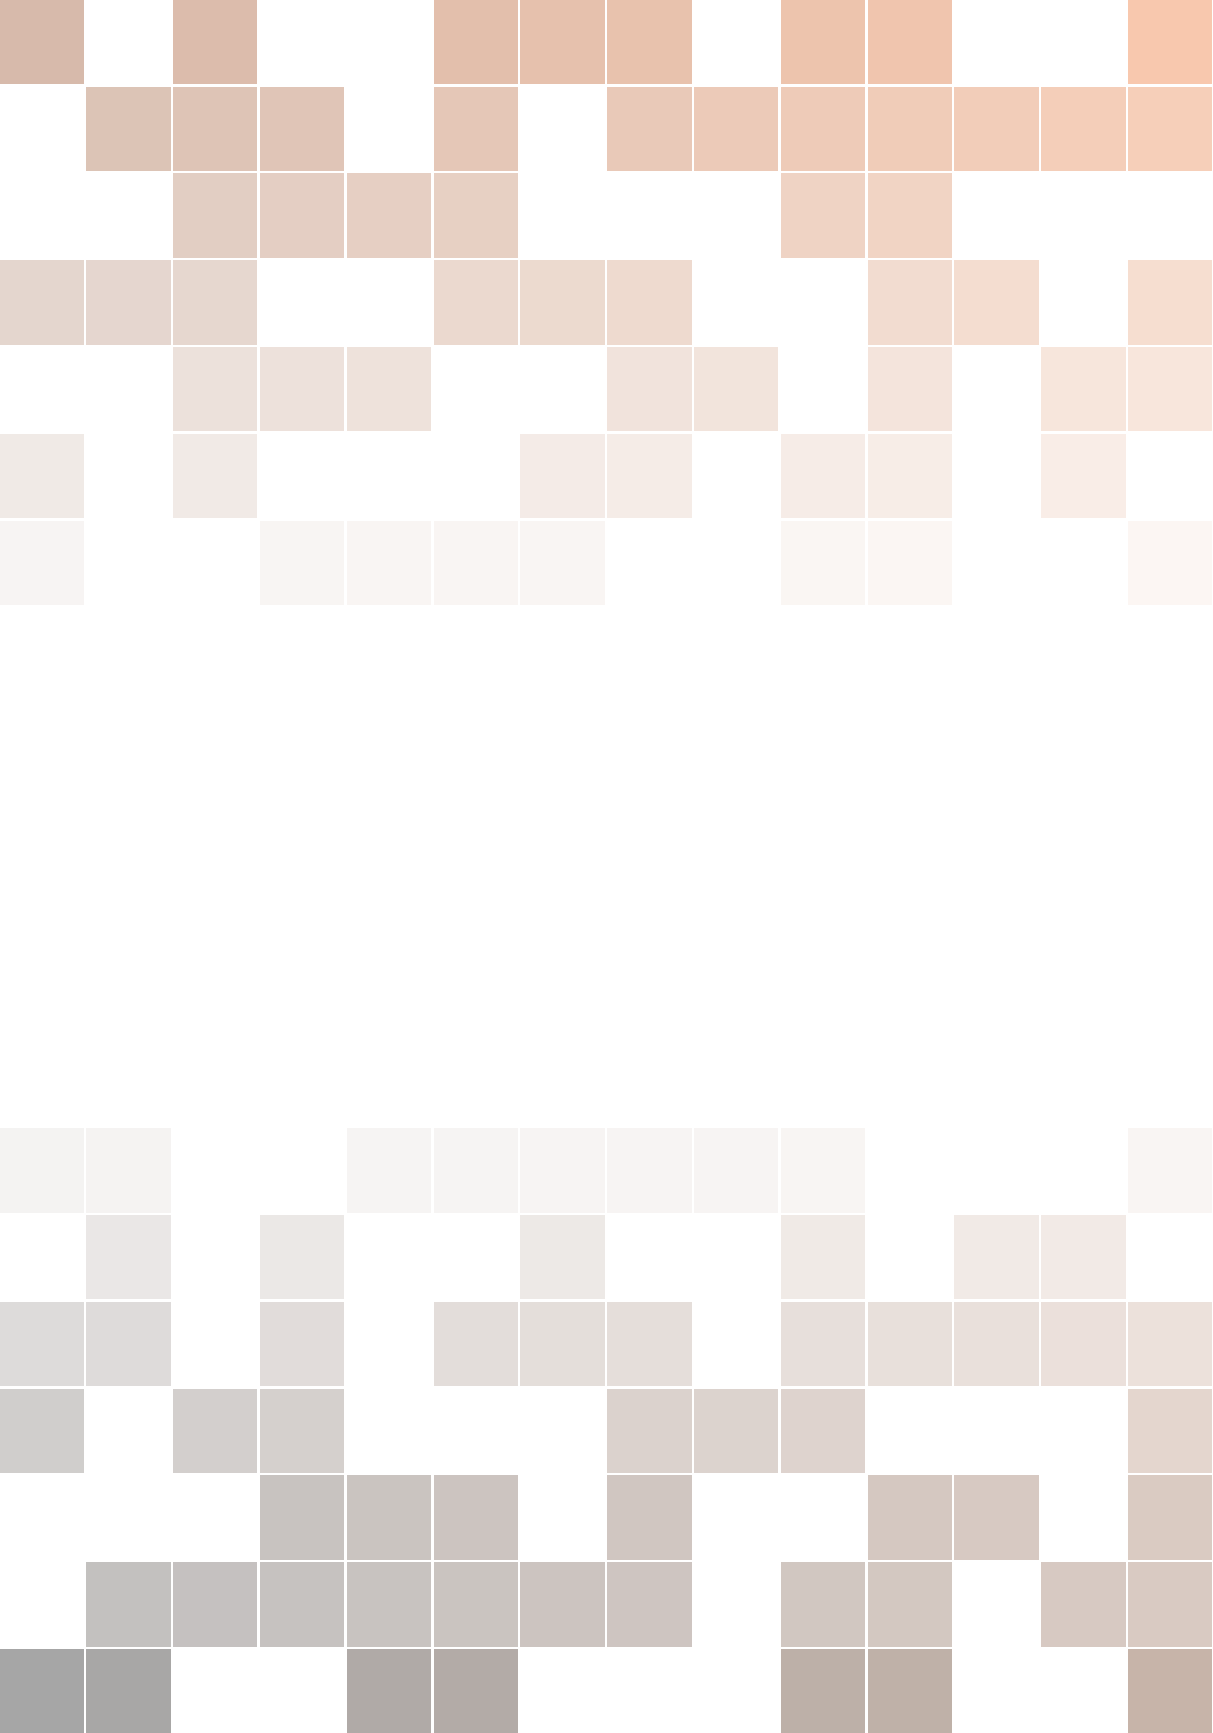
\includegraphics[width=\paperwidth]{background}};
\draw (current page.center) node [fill=ocre!30!white,fill opacity=0.6,text opacity=1,inner sep=1cm]{%
\parbox[c][][t]{\paperwidth}{%
\centering\bfseries\sffamily%
{\Huge \mytitle}\\[15pt]
{\Large \mysubtitle}\\[20pt]
{\huge \myauthorname}\\[15pt]
{\large \mydate}
}% end parbox
};
\end{tikzpicture}
\vfill
\endgroup

%----------------------------------------------------------------------------------------
%	COPYRIGHT PAGE
%----------------------------------------------------------------------------------------

\newpage
~\vfill
\thispagestyle{empty}

\noindent Copyright \copyright\ 2017 \myauthorname\\

\noindent \textsc{Release:\gitRels (\mydate)}\\

% \noindent \textsc{book-website.com}\\ % URL

\noindent Licensed under the Creative Commons Attribution-NonCommercial 3.0 Unported License (the ``License''). You may not use this file except in compliance with the License. You may obtain a copy of the License at \url{http://creativecommons.org/licenses/by-nc/3.0}. Unless required by applicable law or agreed to in writing, software distributed under the License is distributed on an \textsc{``as is'' basis, without warranties or conditions of any kind}, either express or implied. See the License for the specific language governing permissions and limitations under the License.\\ % License information

% \noindent \textit{First printing, March 2013} % Printing/edition date

\chapterimage{chapter_head_2.pdf}
\chapter*{Forord} 

Dette kompendiet er ment som et tillegg til boka 
\href{http://www2.tisip.no/boker/ltj/}{Linux tjenestedrift} \cite{book:linux_tjenestedrift}
skrevet av Mads E. Eilertsen og Arne B. Mikalsen, utgitt 2003. Kompendiet er ikke spesielt nyttig alene, men
noen tips og forklaringer står seg nok på egenhånd.

Emnet IBE115 Serverdrift som jeg underviser ved \href{http://www.himolde.no/}{Høgskolen i Molde}, bruker
boka Linux tjenestedrift som pensum fordi det er den eneste boka om temaet på norsk.
Grunnen til at jeg har skrevet kompendiet er at boka åpenbart er utdatert når det kommer til informasjon 
om programvare. Jeg har tidligere publiserte mange individuelle tips til studentene. Dette kompendiet
samler disse tipsene og mer på et sted i ett lett søkbart format.

\begin{center}
Molde, høsten 2017\\
Hans Fredrik Nordhaug\\
\href{mailto:hansfn@gmail.com}{hansfn@gmail.com}
\end{center}




%----------------------------------------------------------------------------------------
%	TABLE OF CONTENTS
%----------------------------------------------------------------------------------------

\pagestyle{empty} % No headers
\tableofcontents % Print the table of contents itself
\cleardoublepage % Forces the first chapter to start on an odd page so it's on the right
\pagestyle{fancy} % Print headers again

%----------------------------------------------------------------------------------------
%	CONTENT
%----------------------------------------------------------------------------------------

\part{Generelt}
\chapter{Linux}\index{Linux} % kommandolinja og sentrale verktøy

Linux er kjernen til operativsystemet som vanligvis går under samme navn. Skal man være
helt korrekt bør operativsystemet kalles \textbf{GNU/Linux}\index{Linux!GNU/Linux} 
fordi userland kommer fra \href{https://www.gnu.org/}{GNU-prosjektet}
som er drevet av \href{https://www.fsf.org/}{Free Software Foundation (FSF)}.

Det viktigste å huske er at hele Linux-operativsystemet (eller GNU/Linux om du vil) er 
\href{https://en.wikipedia.org/wiki/Free_and_open-source_software}{fri og åpen programvare (FOSS)}.
Husk at fri og åpen programvare ikke bare betyr at det er gratis, som jo er en stor fordel, men 
også at du kan endre og tilpasse programvaren. Dette gjør at Linux har fått en voldsom utbredelse
og brukes i alt fra ordinære servere og nettverksutstyr, 
\href{https://en.wikipedia.org/wiki/Internet_of_things}{IOT}-utstyr, mobiltelefoner, bilen din, 
kjøleskapet ditt \dots Linux fungerer også flott som vanlig PC, men det er ikke den vanligste 
bruken.

GNU/Linux er svært moden programvare. Utviklingen av GNU startet allerede 1983, og første utgave 
av Linux ble sluppet i 1991 av finnen Linus Torvalds som fortsatt styrer utvikling av Linux.
Vil du vite mer om Linux, så er 
\href{https://en.wikipedia.org/wiki/Linux}{Linux-artikkelen på Wikipedia} \cite{wiki:linux}
en god start.

\section{Administratortilgang}\index{root}\index{sudo}

For å kunne administrere serveren din i dette emnet (og eventuelt seinere i arbeidslivet) 
trenger du administratortilgang. Superbrukeren på en Linux-server heter \file{root}, og du
trenger denne kontoen sitt passord for å kunne logge inn. Dette er en stor ulempe hvis flere
skal administrere serveren - du vet ikke hvem som logget inn og du kan heller ikke endre 
\file{root}-passordet utenat det påvirker de andre.

Den vanligste løsning på dette problemet er å bruke \prog{sudo} - \textquote{super user do}. 
Hvis du får sudo-tilgang, så kan du utføre kommandoer som om du var \file{root} uten at du
trenger å logge inn som \file{root}. \prog{sudo} spør om ditt passord - og husker det en stund
slik at du slipper å skrive passordet hele tiden. En ekstra fordel med \prog{sudo} er at
du kan gi en bruker bare delvis administratortilgang. 

Hvis du trenger å være \file{root} over en lengre periode, så kan du bruke 

\cmd[\$]{sudo su -} 

til å bli brukeren \file{root}. Du hopper tilbake til din egen bruker med \prog{exit}.
Faren ved å være \file{root} hele tiden, er at du kan gjøre stor skade uten at du er klar over
det. Skriver du alltid sudo så blir du litt oppmerksom på at du har superkrefter.

\begin{remark}
Jeg har droppet sudo fra kommandolinje-eksemplene i dette kompendiet. Jeg bruker altså

\cmd{service apache2 reload}

istedenfor

\cmd[\$]{sudo service apache2 reload}

Dette er selvfølgelig bare latskap. Legg også merke til at kommandolinja starter 
med \# når jeg er \file{root} og \$ når jeg er en ordinære bruker. 
Du kan sjekke hvem du er med \prog{whoami} ...
\end{remark}

 % Linux - kommandolinja og sentrale verktøy
\chapter{Kapittel to}

\section{Tema 2}\index{Tema 2}

\section{Definitions}\index{Definitions}

This is an example of a definition. A definition could be mathematical or it could define a concept.

\begin{definition}[Definition name]
Given a vector space $E$, a norm on $E$ is an application, denoted $||\cdot||$, $E$ in $\mathbb{R}^+=[0,+\infty[$ such that:
\begin{align}
& ||\mathbf{x}||=0\ \Rightarrow\ \mathbf{x}=\mathbf{0}\\
& ||\lambda \mathbf{x}||=|\lambda|\cdot ||\mathbf{x}||\\
& ||\mathbf{x}+\mathbf{y}||\leq ||\mathbf{x}||+||\mathbf{y}||
\end{align}
\end{definition}

%------------------------------------------------


%------------------------------------------------

\section{Remarks}\index{Remarks}

This is an example of a remark.

\begin{remark}
The concepts presented here are now in conventional employment in mathematics. Vector spaces are taken over the field $\mathbb{K}=\mathbb{R}$, however, established properties are easily extended to $\mathbb{K}=\mathbb{C}$.
\end{remark}

%------------------------------------------------


\section{Examples}\index{Examples}

This is an example of examples.

\subsection{Equation and Text}\index{Examples!Equation and Text}

\begin{example}
Let $G=\{x\in\mathbb{R}^2:|x|<3\}$ and denoted by: $x^0=(1,1)$; consider the function:
\begin{equation}
f(x)=\left\{\begin{aligned} & \mathrm{e}^{|x|} & & \text{si $|x-x^0|\leq 1/2$}\\
& 0 & & \text{si $|x-x^0|> 1/2$}\end{aligned}\right.
\end{equation}
The function $f$ has bounded support, we can take $A=\{x\in\mathbb{R}^2:|x-x^0|\leq 1/2+\epsilon\}$ for all $\epsilon\in\intoo{0}{5/2-\sqrt{2}}$.
\end{example}

\subsection{Paragraph of Text}\index{Examples!Paragraph of Text}

\begin{example}[Example name]
\lipsum[2]
\end{example}

%------------------------------------------------

\section{Exercises}\index{Exercises}

This is an example of an exercise.

\begin{exercise}
This is a good place to ask a question to test learning progress or further cement ideas into students' minds.
\end{exercise}

%------------------------------------------------

\section{Problems}\index{Problems}

\begin{problem}
What is the average airspeed velocity of an unladen swallow?
\end{problem}

%------------------------------------------------

\section{Vocabulary}\index{Vocabulary}

Define a word to improve a students' vocabulary.

\begin{vocabulary}[Word]
Definition of word.
\end{vocabulary}


 % Programvareinstallasjon
\chapterimage{chapter_head_1.pdf} % Chapter heading image

\chapter{Læreboka}

\section{Table}\index{Table}

\begin{table}[h]
\centering
\begin{tabular}{l l l}
\toprule
\textbf{Treatments} & \textbf{Response 1} & \textbf{Response 2}\\
\midrule
Treatment 1 & 0.0003262 & 0.562 \\
Treatment 2 & 0.0015681 & 0.910 \\
Treatment 3 & 0.0009271 & 0.296 \\
\bottomrule
\end{tabular}
\caption{Table caption}
\end{table}

%------------------------------------------------

\section{Figure}\index{Figure}

\begin{figure}[h]
\centering
\includegraphics[scale=0.5]{placeholder}
\caption{Figure caption}
\end{figure}
 % Læreboka

\part{Programvare}
\chapterimage{chapter_head_1.pdf}
\chapter{Apache / HTTP / Web}\index{Apache}  % kapt 4

Dokumentasjonen for siste/gjeldende utgave av Apache finner
du alltid på\\ \url{http://httpd.apache.org/docs/current/}

I dette kapitlet vil vi vise til diverse informasjon for 
utgave 2.4 og dermed istedenfor lenke til\\
\url{http://httpd.apache.org/docs/2.4/} \cite{docs:apache}

\section{Installasjon}

Som vanlig installerer man (Apache) med \prog{apt}

\cmd{apt install apache2}

Jada, det funger fortsatt/også med \prog{apt-get} hvis du er vant til det.

Hvis du har lyst til å leke litt med PHP (og seinere installere Wordpress
eller et annet PHP-basert CMS), så kan du installere PHP-støtte i Apache med

\cmd{apt install libapache2-mod-php}\index{PHP}

Dette legger til en PHP-modul i Apache som er den vanligste måten å kjøre PHP på.

Et annet alternativ som er ganske vanlig hos en del hostingselskaper 
er FastCGI-modulen sammen med PHP-FPM.

\section{Konfigurasjon}

Som tidligere påpekt bruker læreboka Apache 2.2, mens vi skal bruke Apache 2.4. 
Dette er standardvalget i Debian og gjeldene utgave for Apache. Før vi tar
noen spesifikke detaljer, merk at:

\begin{remark}
Læreboka snakker om \file{httpd.conf}\index{httpd.conf} som Apache sin konfigurasjonsfil. 
Den samme fila heter \file{apache2.conf}\index{apache2.conf} i Debian og ligger selvfølgelig i 
mappa \file{/etc/apache2/}. Før du starter med denne oppgaven bør du lese starten 
av \file{apache2.conf} (på din server) - bruk less. Du vil da skjønne at 
fila \file{apache2.conf} er satt sammen av flere filer. Dette er istedenfor at 
all konfigurasjon er samlet i en \textquote{gigantisk} fil.
\end{remark}

\subsection{Overgang fra 2.2 til 2.4}

Dette er godt beskrevet i dokumentet
\href{http://httpd.apache.org/docs/2.4/upgrading.html}{Upgrading to 2.4 from 2.2}.
Du må lese om \textquote{Access control} som viser hvordan man setter opp
tilgangskontroll i Apache 2.4. Dette er altså en korreksjon til kapittel 4.8 
i lærebok. I svært korte trekk kan man si at \config{Order}, \config{Allow} og \config{Deny}
er byttet ut med \config{Require}\index{Apache!direktiver!Require}\index{Require|see{Apache, direktiver}}.

\subsection{Direktiver}

Apache blir styrt gjennom såkalte direktiver i konfigurasjonsfilene. Alle direktivene 
er godt dokumentert, med eksempler, i Apache sin dokumentasjon - se
\href{http://httpd.apache.org/docs/2.4/mod/quickreference.html}{Directive Quick Reference}.
Etterhvert som man vet omtrent hva direktivene heter, så trenger man ikke mer
enn denne oversikten. 

Den kanskje kraftigste funksjonaliteten til Apache finner man i modulen Rewrite.
\index{Apache!moduler!Rewrite}\index{Rewrite|see{Apache, moduler}}\index{mod\_rewrite|see{Apache, moduler}}
Denne blir ikke omtalt i læreboka, men dere kan lese om dette i håndboken
\href{http://httpd.apache.org/docs/2.4/rewrite/}{URL Rewriting with mod\_rewrite}.

En annen nyttig modul er UserDir som lar deg sette opp hjemmesider for hver enkelt
bruker på serverene. Dere kan lese mer om UserDir i howto-en
\href{http://httpd.apache.org/docs/2.4/howto/public\_html.html}{Per-user web directories}.
\index{Apache!direktiver!UserDir}\index{Apache!moduler!UserDir}
\index{UserDir|see{Apache, Moduler}}\index{mod\_userdir|see{Apache, moduler}}

\section{Trafikkanalyse}\index{trafikkanalyse}\index{logganalyse}

Når man driver et nettsted er det viktig å vite så mye som mulig om de besøkende.
Tidligere ble dette gjort ved å se på loggfilene til webserveren (Apache). Kjente 
programmer for dette er Webalizer og AWStats.\index{Webalizer}\index{AWStats}

Moderne analyseverktøy baserer seg på sporing på klientsiden (i nettleseren) ved
hjelp av JavaScript. Den meste kjente løsningen er Google Analytics. Hvis du 
ønsker å ha fullkontroll over dataene dine eller lovgivning sier at du ikke kan bruke 
en tredjepart til å samle inn data, så er løsningen Piwik.\index{Piwik}
Jeg anbefaler at dere tester det ut hvis dere får tid. 
(Piwik fins for tiden dessverre ikke som en offisiell Debian-pakke.)

 % Apache / HTTP / Web                              kapt 4
\chapter{Samba / SMB / Fildeling} % kapt 3
 % Samba / SMB / Fildeling                          kapt 3
\chapter{Qmail}\index{Qmail} % kapt 5

Før du leser dette kapitlet så er det lurt å ha sett eller i det minst bland gjennom
forelesningen om Qmail. Jeg gjentar ikke alt som står forelesningen her.

I læreboka kapittel 5.10.2-5.10.9 omtales (manuell) installasjon og konfigurering av 
\prog{qmail}, \prog{daemontools} og \prog{ucspi-tcp}. Dette kan dere se helt bortifra.
Vi skal selvfølgelig bruke Apt.

Testing av Qmail, som utføres i 5.10.6, er gjengitt her i kompendiet. Jeg anbefaler
at disse testene utføres. Jeg anbefaler også at dere tester å \textquote{snakke}
SMTP ved hjelp av \prog{telnet} - se 5.10.9 i læreboka eller opptak fra forelesning.

Ellers kan \href{http://www.lifewithqmail.org/lwq.html}{Life with Qmail} være en god ressurs
for å lære om Qmail (hvis man ikke har læreboka).

\begin{remark}
Aliaser og alias-brukerens spesielle roller blir omtalt i neste kapittel.
\end{remark}


\section{Installasjon}

På grunn av en (fersk) feil i pakken \prog{qmail-run} så må vi installere Daemontools 
først:

\cmd{apt install daemontools-run}

Etterpå kan du installere Qmail. Vi installerer pakken \prog{qmail-run} slik at 
Qmail automatisk bruker Daemontools.

\cmd{apt install qmail-run}

Etter dette kjører Qmail - din server kan sende og motta epost. Du kan ikke bruke 
den vanlige \prog{service}-kommandoen for Qmail siden den er kontrollert av 
Daemontools. I tillegg til Daemontools-kommandoene så fins det \prog{qmailctl}.
Hvis du lurer på om Qmail faktisk kjører, bruk

\cmd{qmailctl stat}\index{qmailctl|see{Qmail}}\index{Qmail!qmailctl}

Hvis du skal lese epost lokalt på serveren, så anbefaler jeg programmet \prog{mutt}. 
Dette minner ikke mye om Outlook eller G-mail, men du klarer nok å lese og sende epost.
Du installerer det som vanlig med

\cmd{apt install mutt}

\section{Konfigurasjon}

\subsection{Daemontools}\index{Daemontools}

\begin{remark}
Service-mappa i Debian er \file{/etc/service} i motsetning til
læreboka som bruker \file{/service}. Prøv å huske det ...
\end{remark}

Daemontools er en samling verktøy for å administrere tjenester (services).
I motsetning til Systemd, så overvåker Daemontools tjenestene og starter 
dem på nytt hvis de dør. Dette er meget praktisk.

For å administrere en tjeneste oppretter man en mappe i \file{/etc/service}
som inneholder en fil \file{run} som starter tjenesten. Resten er automagisk.

Pakken \prog{qmail-run} oppretter \file{/etc/service/qmail-smtpd} (og to andre mapper)
som gjør at Qmail blir kontrollert Daemontools.

Daemontools har egentlig bare to kommandoer - \prog{svstat} som gir status for en tjeneste
og \prog{svc} som kontrollerer tjenesten.
\index{svstat|see{Daemontools}}\index{Daemontools!svstat}
\index{svc|see{Daemontools}}\index{Daemontools!svc}

Med \prog{qmail-smtpd} som et eksempel har du følgende nesten selvforklarende eksempler:

\cmd{svstat /etc/service/qmail-smtpd}\\
\cmd{svc -u /etc/service/qmail-smtpd}\\
\cmd{svc -p /etc/service/qmail-smtpd}

Hvis du lurer på hva de to siste eksemplene gjør, les man-siden:

\cmd[\$]{man svc}

\subsection{Kontrollfiler}

Alle datafilene til Qmail ligger i \file{/var/lib/qmail/}. Legg merke til 
at hjemmeområdet til \file{alias}-brukeren er i samme mappe - \file{/var/lib/qmail/alias/}.

Kontrollfilene er tilgjengelig i \file{/etc/qmail}. (\file{/var/lib/qmail/control} er en symbolsk
lenke til \file{/etc/qmail}.) 

De viktigste filene er \file{me}, \file{locals} og \file{rcpthosts}. Du finner informasjon 
om kontrollfilene i man-sidene for \prog{qmail-smtpd} og \prog{qmail-inject}. For en komplettliste
av kontrollfiler kjør:

\cmd[\$]{man qmail-control}

\section{Testing}

I de følgende testene/eksemplene skal du bytte ut \file{minbruker} med ditt brukernavn.
Målet med testene er å skjønne hvordan Qmail fungerer. Du sender selvfølgelig vanligvis
epost via en MUA/epostklient (som \prog{mutt}) - ikke via \prog{qmail}-kommandoer.

\begin{remark}
Standard innboks for en bruker i Debian er \file{/var/mail/brukernavn} i motsetning
til læreboka som bruker \file{/home/brukernavn/Mailbox}.

\end{remark}

Loggfilen for alle testene er \file{/var/log/qmail/current}. Hvis du ønsker å se filen
med forståelig tidsstempel, bruk

\cmd{cat /var/log/qmail/current | tai64nlocal}

Ofte ønsker du bare å se de f.eks. 7 siste linjene i loggfilen:

\cmd{cat /var/log/qmail/current | tail -n 7 | tai64nlocal}

NB! Loggfilen for innkommende (ekstern) epost er \file{/var/log/qmail/smtpd/current}

\subsection*{Testmelding til lokal adresse}

Sender en melding som kun har et \textquote{to}-felt og ingen kropp.

\cmd[\$]{echo \textquotedbl{}to: minbruker\textquotedbl{} | qmail-inject}

Sjekk loggen og brukerens innboks (enten med \prog{nano} eller \prog{mutt}).

\subsection*{Testmelding til ukjent lokal adresse}

\cmd[\$]{echo \textquotedbl{}to: brukersomikkefins\textquotedbl{} | qmail-inject}

Sjekk loggen og brukerens innboks (enten med \prog{nano} eller \prog{mutt}).
Legg merke til Bounce-meldingen siden adressen ikke fantes.

\subsection*{Testmelding til postmaster}

\cmd[\$]{echo \textquotedbl{}to: postmaster\textquotedbl{} | qmail-inject}

Sjekk loggen. Hvor havner eposten?

\subsection*{Testmelding til ekstern adresse}

Bruk din vanlige epostadresse i denne testen.

\cmd[\$]{echo \textquotedbl{}to: deg@etellerannetdomene\textquotedbl{} | qmail-inject}

Sjekk loggen.

\subsection*{Testmelding til ukjent avsender og ukjent mottaker}

\cmd[\$]{echo \textquotedbl{}to: ukjentmottaker\textquotedbl{} | qmail-inject -f ukjentavsender}

Sjekk loggen. Legg merke til dobbel Bounce-meldingen siden også avsenderadressen 
ikke fantes.
 % Qmail (Exim eller Postfix) / SMTP / E-post       kapt 5
\chapter{ezmlm / - / E-post: Aliaser og lister} % kapt 6
 % ezmlm / - / E-post: Aliaser og lister            kapt 6
\chapter{Dovecot} % kapt 7

\section{Installasjon}

Lærebok bruker \prog{qmail-pop3d} og \prog{qpopper}. Dessverre kan 
ingen av disse brukes.

\begin{itemize}
\item \prog{qmail-pop3d} kan ikke brukes fordi programmet checkpassword ikke 
   virker. (Ref kap. 7.3)
\item \prog{qpopper} kan ikke brukes fordi det ikke lenger vedlikeholdes og 
   det er heller ikke tilgjengelig for Debian. (Ref kap. 7.5)
\end{itemize}

Det er mange andre muligheter (som jeg lister opp i forelesningen),
men jeg tror det er minst arbeid å prøve Dovecot sin POP3. 

\cmd{apt install dovecot-pop3d}

Endre konfigurasjonen for Dovecot slik at det fungerer uten noe problemer.
Opprett fila \file{/etc/dovecot/local.conf} med følgende to linjer:

\begin{filedata}
disable_plaintext_auth = no
mail_access_groups = mail
\end{filedata}

Få Dovecot til å lese konfigurasjonen på nytt. OK, hvis du lurer
så er det selvfølgelig
   
\cmd{service dovecot reload}

\section{Testing av POP3}

Jeg syns det er lurt at dere prøver POP3 på protokollnivå (med
telnet) slik som vi gjorde med HTTP og SMTP. Bruk

\cmd[\$]{telnet lpcXYZ.himolde.no pop3}

Denne kommandoen kan du kjøre som deg selv (uten \prog{sudo}).
Aller best er det hvis du gjør det fra en annen maskin 
(f.eks ibe101.himolde.no) slik at du er helt sikker på at det virker.

Prøv gjerne fra din egen PC også med f.eks. 
\href{https://www.mozilla.org/nb-NO/thunderbird/}{Thunderbird}

\begin{remark}
Siden vi kjører POP3 uten kryptering anbefaler jeg at du 
legger til en egen testbruker for POP (med \prog{adduser}).
\end{remark} % Dovecot / POP3, IMAP / E-post: Aksessprotokoller kapt 7
\chapter{Bind, tinydns og dnscache} % kapt 8
% #################################

\index{Bind}\index{djbdns}
\index{tinydns|see{djbdns}}\index{djbdns!tinydns}
\index{dnscache|see{djbdns}}\index{djbdns!dnscache}

Et lite tips: Ikke installer Bind før du har gjort deg ferdig med
dnscache og tinydns. Bind, hvis du ikke endrer konfigurasjonen, vil
lytte på alle IP-adresser etter installasjon og komme i konflikt med
dnscache og tinydns.
 
% ####################
\section{Installasjon}
% ####################

Installasjon av Bind fungerer som standard og vil ikke bli omtalt her. 
Du må bare husk at pakken heter \file{bind9}. Vi skal fokuserer på djbdns nedenfor.

Akkurat som for Ezmlm, så fins det ingen pakke for djbdns i den stabile utgaven av Debian som vi bruker.
Dessverre fins det ikke lenger noen pakke for andre utgaver av Debian heller. 
På \url{https://packages.debian.org/djbdns} finner du bare en pakke for arm64-prosessoren. 
Vi må derfor bruke et skittent triks:

Laste ned pakken fra \url{http://snapshot.debian.org/}

Installasjon av pakker fra \url{http://snapshot.debian.org/} fungerer greit fordi 
pakken blir registrert av pakkesystemet, og alle avhengigheter blir behandlet som vanlig. 
Generelt kan man ikke regne med at pakker fra snapshots.debian.org fungerer siden avhengigheter
kan mangle.

Du finner mulige pakker via \url{http://snapshot.debian.org/package/pakkenavn/}, altså 
\url{http://snapshot.debian.org/package/djbdns/}. På den siden vil du etterhvert finne riktig
deb-fil for i386:

\file{http://snapshot.debian.org/archive/debian/20130529T040126Z/pool/main/d/djbdns/djbdns\_1.05-9\textasciitilde{}exp2\_i386.deb}

Kopier URL-en over og last ned med \prog{wget}. 
Deretter installerer du manuelt for eksempel med:

\cmd{dpkg -i djbdns\_1.05-9\textasciitilde{}exp2\_i386.deb}

% ############################################
\section{Konfigurasjon av dnscache og tinydns}
% ############################################

\index{djbdns!tinydns}
\index{djbdns!dnscache}
\index{dnscache-conf|@see{djbdns}}\index{djbdns!dnscache-conf}
\index{tinydns-conf|@see{djbdns}}\index{djbdns!tinydns-conf}


Vi skal konfigurere dnscache og tinydns fra grunnen av - som beskrevet i læreboka (for en gangs skyld).
Når vi installerte Qmail, slapp vi billig unna. Pakken \file{qmail-run} installerer for eksempel 
\file{qmail-uids-gids} som oppretter brukere. Vi må gjøre dette selv:

\cmd{useradd -s /bin/false Gdnscache}\\
\cmd{useradd -s /bin/false Gtinydns}\\
\cmd{useradd -s /bin/false Gdnslog}

PS! Du kan ikke logge inne som disse brukerne siden de har \prog{/bin/false} som SHELL. 

Siden det ikke fins en \file{djbdns-run} pakke så må vi også opprette run-filer osv. for Daemontools.
Heldigvis fins det verktøy for dette. Vi må bruke \prog{dnscache-conf} og \prog{tinydns-conf}.
Det viktigste med disse kommandoene er å benytte riktig IP-adresser.

For å sette opp dnscache som en lokal tjeneste (standard), bruk

\cmd{dnscache-conf Gdnscache Gdnslog /etc/dnscache}

For å sette opp tinydns som en offentlig tjeneste, bruk

\cmd{tinydns-conf Gtinydns Gdnslog /etc/tinydns 158.38.74.XYZ}

Ja, du må bytte ut \textquote{XYZ} med ditt lpc-nummer.
 
For å starte dnscache eller tinydns som en tjeneste, lenker 
du bare opp disse mappene i \file{/etc/service}.
Du kan sjekke med \prog{svstat} (etter noen sekunder).

\cmd{ln -s /etc/dnscache /etc/service}\\
\cmd{svstat /etc/service/dnscache}

\cmd{ln -s /etc/tinydns /etc/service}\\
\cmd{svstat /etc/service/tinydn}

% ##########################################
\subsection{Legge til ressursdata i tinydns}
% ##########################################

\index{djbdns!tinydns}

Dette er omtalt i lærebok på side 243 og utover. Jeg gjengir i korte trekk her.

For å legge til ressursdata så må du være i mappa \file{/etc/tinydns/root/}.
Det er i alle fall mye enklere ... Hver gang du har lagt til ressursdata, 
må du kompilere data-filen slik at tinydns ser endringen. Dette gjør du med 

\cmd{make}

Kanskje du må installere \file{make}-pakken?

For å legge til navnetjenere, NS-oppføringer, bruk:

\cmd{./add-ns lpcXYZ.himolde.no Offentlig-IP}\\
\cmd{./add-ns lpcXYZ.himolde.no IP-alias}

For å legge til domenenavn, A-oppføringer, bruk:

\cmd{./add-host lpcXYZ.himolde.no Offentlig-IP}

For å legge til et domenenavn til for samme IP (alias), bruk:

\cmd{./add-alias somename.lpcXYZ.himolde.no Offentlig-IP}

Dette gir ikke en vanlig CNAME-oppføring.

Alle disse \file{add}-kommandoene er egentlig bare wrappere rundt
\prog{tinydns-edit}. Du kan derfor slå opp i man-siden for dette programmet
hvis du lurer på noe.
\index{tinydns-edit|@see{djbdns}}\index{djbdns!tinydns-edit}

% #############################
\section{Konfigurasjon av Bind}
% #############################

\index{Bind}

Dokumentasjonen til gjeldende utgave av Bind finner du alltid på\\
\url{https://www.isc.org/downloads/bind/doc/} \cite{docs:bind}\\
Debian bruker for øyeblikket utgave 9.10 av Bind.

Et klassisk eksempel på sonefile finner du på\\
\url{http://www.zytrax.com/books/dns/ch6/mydomain.html}\\
Alle ressursdata for et domene legges inn i sonefila.

\begin{remark}
Selv om læreboka nevner det, så trenger du altså ikke legge til brukere osv 
som du gjorde for dnscache og tinydns. Du trenger heller ikke opprette mapper eller noe annet.
Bind fungerer ut av boksen.
\end{remark}

Legg spesielt merke til at Bind sin konfigurasjon i Debian ligger i \file{/etc/bind}, 
ikke \file{/etc/bind9} (som ville vært logisk siden pakken heter \file{bind9}) 
eller \file{/etc/named}. 

Kommentarene nedenfor er rettet mot arbeidet med den obligatoriske oppgaven
om DNS. Ikke alt har generell gyldig. Jeg forutsetter også at du har lagt
til et IP-alias for nettverkskortet ditt, slik at du har to offentlige IP-adresser
for serveren din. 

Du bør endre \file{/etc/bind/named.conf.options} før du setter i gang.
For å spare dere litt forvirring bør dere slå av rekursjon og få Bind til å lytte 
på en annen offentlig IP enn tinydns. Bruk:

\begin{filedata}
recursion no;
listen-on \{ 158.38.74.ZYX; \};
listen-on-v6 \{ none; \};
\end{filedata}

Dette er omtalt nederst på side 253 i læreboka. 

En naturlig plassering for sonefilen for ditt domene er 
\file{/etc/bind/db.lpcXYZ.himolde.no}.  
Du legger til sonen i fila \file{/etc/bind/named.conf.local}. 
Du kan se i \file{/etc/bind/named.conf.default-zones} for 
å lære hvordan du gjør det. Hvis 

\cmd{service bind9 reload}

ikke virker som forventer, stopper og starter du bare tjenesten.

For å feilsøke Bind konfigurasjonen så har du to verktøy: \\ 
\prog{named-checkconf} og \prog{named-checkzone}.
\index{named-checkconf|@see{Bind}}\index{Bind!named-checkconf}
\index{named-checkzone|@see{Bind}}\index{Bind!named-checkzone}

For å sjekke selve konfigurasjonen (utenom sonefilene eller ressursdata om du vil), bruk:

\cmd{named-checkconf} 

For å sjekke en sonefil (og dens ressursdata), bruk:

\cmd{named-checkzone lpcXYZ.himolde.no /etc/bind/db.lpcXYZ.himolde.no}

% ######################################################
\section{Læreboka og den obligatoriske oppgaven}
% ######################################################

Når læreboka snakker om \textquote{z.example.com} (første gang på side 243),
så bytter du det ut med ditt domene - \textquote{lpcXXX.himolde.no}. Det er litt 
mer naturlig.

Som det står i oppgaveteksten skal Bind ha samme ressursdata som
tinydns. Du skal altså \textbf{ikke} delegere autoritet for et barnedomene fra
tinydns til bind - ref 8.5.3 i læreboka.

Hvis du lurer på hvilke tjenester (eller prosesser)
som lytter på port 53 (DNS), bruk

\cmd{netstat -anp | grep \tqs:53 \tqs}

% ##############################################
\section{IP-alias og den obligatoriske oppgaven}
% ##############################################

Læreboka anbefaler at vi oppretter en egen IP-adresse (IP-alias) for tinydns, 
men det er ikke nødvendig. Vi kan bruke vår offentlige IP siden dnscache kun bruker localhost.
Derimot trenger vi et IP-alias for Bind slik at det ikke blir konflikt med tinydns.
For å unngå konflikter med andre på labnettet, så skal du bruke et IP-alias
som er 60 høyere enn den offentlige IP-adresse. Med andre ord, hvis du 
har f.eks. 158.38.74.192, så skal IP-aliaset være 158.38.74.252.

Et nettverkskort kan han mange forskjellige IP-adresser på samme inngang. 
Det er en hovedadresse og resten kaller vi aliaser. 
Statiske nettverk, uten DHCP, krever at vi konfigurerer 
serveren i filen \file{/etc/network/interfaces}. 

\index{ifconfig}\index{ip}
Bruk \prog{ifconfig} eller \prog{ip} for å se på gjeldende, aktive nettverksinnstillinger.
Dere vil se at nettverkskortet heter \file{ens192}, ikke \file{eth0} som det pleide 
å hete tidligere. Disse nye navnene gir ekstra informasjon om kortet.

For å opprette et IP-aliaset fra eksemplet over veldig kjapt, kan vi bruke

\cmd{ifconfig ens192:1 158.38.74.252 netmask 255.255.255.128}

Ulempen med å gjøre det kjapt og enkelt er at IP-aliaset forsvinner når maskiner starter
på nytt. Det er derfor bedre å legge det til i selve konfigurasjonen.
På slutten av \file{/etc/network/interfaces} legg til

\begin{filedata}
auto ens192:0
allow-hotplug ens192:0
iface ens192:0 inet static
        address 158.38.74.252
        netmask 255.255.255.128
\end{filedata}

for å definere IP-aliaset fra eksemplet over. Du kan aktivere IP-aliaset med

\cmd{ifup ens192:0}

Du skjønner da at det også fins en kommando \prog{ifdown}. % Bind, tinydns og dnscache / DNS / Navnetjeneste  kapt 8
\chapter{ProFTP / FTP / Filoverføring} % kapt 10
 % ProFTP / FTP / Filoverføring                     kapt 10
\chapter{Nextcloud / Filsynkronisering}
 % Nextcloud / Filsynkronisering

\part{Litt av hvert}
\chapter{Skripting} 										
 % Skripting
\chapter{Diverse om sikkerhet} % kapt 11 % Diverse om sikkerhet                             kapt 11
\chapter{Operativsystem, prosesser og filsystem}
 % Operativsystem, prosesser og filsystem

%----------------------------------------------------------------------------------------
%	BIBLIOGRAPHY
%----------------------------------------------------------------------------------------

\chapter*{\bibname}
\addcontentsline{toc}{chapter}{\textcolor{ocre}{\bibname}}
\section*{Bøker}
\addcontentsline{toc}{section}{Bøker}
\printbibliography[heading=bibempty,type=book]
\section*{Nettsteder}
\addcontentsline{toc}{section}{Nettsteder}
\printbibliography[heading=bibempty,type=online]

%----------------------------------------------------------------------------------------
%	INDEX
%----------------------------------------------------------------------------------------

\cleardoublepage
\phantomsection
\setlength{\columnsep}{0.75cm}
\addcontentsline{toc}{chapter}{\textcolor{ocre}{\indexname}}
\printindex

%----------------------------------------------------------------------------------------

\end{document}
